\chapter{Os reagentes organomagnesianos}\label{ch:b1:organomagnesium}

A maioria das moléculas orgânicas úteis tem mais átomos de carbono que
qualquer matéria-prima barata, e o problema central da síntese é unir
dois esqueletos carbônicos por uma nova ligação C--C. Em um composto de
carbono, o carbono é quase sempre o parceiro pobre em elétrons de uma
ligação --- com o oxigênio, com um halogênio --- e dois carbonos pobres
em elétrons não reagem entre si. Na virada do século vinte, um reagente
preparado em um único balão a partir de um haloalcano e de magnésio
inverteu essa situação: seu carbono é rico em elétrons, um \omterm{def:b1:electronic-effects:nucleophile}{nucleófilo} que
ataca o carbono de um grupo carbonila. Com ele, álcoois de quase
qualquer esqueleto podem ser construídos a partir de peças menores. Este
capítulo mostra como o reagente é preparado, por que ele exige um balão
perfeitamente seco, a que ele se adiciona e como planejar com ele.

\begin{recall}
A \omterm{def:b1:periodicity:electronegativity}{eletronegatividade} (\cref{ch:b1:periodicity}); os ácidos e as \omterm{def:b1:lewis-resonance-vsepr:lewis-acid}{bases de
Lewis} e a \omterm{def:b1:lewis-resonance-vsepr:lewis-acid}{ligação dativa} (\cref{ch:b1:lewis-resonance-vsepr}); os
\omterm{def:b1:electronic-effects:nucleophile}{nucleófilos}, os \omterm{def:b1:electronic-effects:nucleophile}{eletrófilos}, as \omterm{def:b1:electronic-effects:curly-arrow}{setas curvas} e a escala de
$\mathrm{p}K_a$ das espécies orgânicas (\cref{ch:b1:electronic-effects});
a classe de um álcool (primário, secundário, terciário) segue a de seu
carbono.
\end{recall}

\section{Preparar um reagente de Grignard}

\begin{definition}[Composto organometálico, reagente de Grignard]\label{def:b1:organomagnesium:organometallic}
Um \emph{composto organometálico}\index{composto organometalico@composto organometálico} contém
pelo menos uma ligação carbono--metal. Um \emph{composto
organomagnesiano}\index{composto organomagnesiano} tem uma ligação C--Mg; o
\emph{reagente de Grignard}\index{reagente de Grignard} \ce{RMgX} (X = Cl, Br, I),
preparado a partir de um haloalcano ou de um haloareno e de magnésio em
um éter, \ce{R-X + Mg -> R-MgX}, é o mais comum.
\end{definition}

O magnésio se insere na ligação C--X. O éter não é um solvente inocente:
o magnésio em \ce{RMgX} tem apenas quatro \omterm{def:b1:quantum-numbers:configuration}{elétrons de valência} à sua
volta, e duas moléculas de éter lhe cedem seus \omterm{def:b1:lewis-resonance-vsepr:lewis}{pares não ligantes},
completando seu octeto e mantendo o reagente em solução.

\begin{omfigure}
\begin{tikzpicture}[font=\small]
  \node (mg) at (0,0) {Mg};
  \node (r) at (-1.5,0) {R};
  \node (x) at (1.5,0) {Br};
  \node (o1) at (0,1.45) {O};
  \node (o2) at (0,-1.45) {O};
  \draw[thick] (r) -- (mg) -- (x);
  \draw[thick, ->, omDef] (o1) -- (mg);
  \draw[thick, ->, omDef] (o2) -- (mg);
  \draw (o1) -- ++(-0.8,0.45) node[left] {\ce{CH3CH2}};
  \draw (o1) -- ++(0.8,0.45) node[right] {\ce{CH2CH3}};
  \draw (o2) -- ++(-0.8,-0.45) node[left] {\ce{CH3CH2}};
  \draw (o2) -- ++(0.8,-0.45) node[right] {\ce{CH2CH3}};
  \node[align=left, anchor=west] at (3.2,0) {duas moléculas de éter cedem\\cada uma um par não ligante (azul):\\magnésio tetraédrico,\\um octeto de elétrons};
\end{tikzpicture}

{\small Um \omterm{def:b1:organomagnesium:organometallic}{reagente de Grignard} em etoxietano (éter dietílico). As
\omterm{def:b1:lewis-resonance-vsepr:lewis-acid}{ligações dativas} oxigênio--magnésio explicam por que o reagente só se
forma em um éter ou em uma \omterm{def:b1:lewis-resonance-vsepr:lewis-acid}{base de Lewis} semelhante.}
\end{omfigure}

\begin{method}[Preparar um reagente de Grignard]\label{met:b1:organomagnesium:prepare}
\begin{enumerate}
  \item Seque toda a vidraria em estufa; equipe o condensador com um tubo
        secante de cloreto de cálcio; use um éter anidro.
  \item Coloque as aparas de magnésio e um pouco de éter em um balão de
        três bocas equipado com condensador, funil de adição e agitador.
  \item Adicione uma pequena porção do haleto; quando a reação começar
        (turvação, ebulição suave do éter), adicione o resto gota a gota,
        a uma velocidade que mantenha um refluxo suave.
  \item Use a solução imediatamente, na mesma aparelhagem seca.
\end{enumerate}
\end{method}

\begin{omfigure}
\begin{tikzpicture}[font=\small]
  \pic at (0,-0.05) {stirrer};
  \pic (f) at (0,0.05) {threeneck={0.35}{omDef!14}};
  \pic at (f-c) {condenser};
  \pic at ($(f-c)+(0,3.2)$) {guardtube};
  \pic[rotate=25] at (f-l) {dropfunnel={0.5}{orange!20}};
  \fill[black!45, rotate around={-25:(f-r)}] ($(f-r)+(-0.17,0)$) rectangle ++(0.34,0.3);
  \draw[->] (2.4,0.9) node[right] {aparas de Mg em éter seco} -- (0.6,0.6);
  \draw[->] (-3.0,3.9) node[left, align=right] {haleto em éter,\\adicionado gota a gota} -- (-1.8,3.4);
  \draw[->] (1.8,5.3) node[right] {condensador (água)} -- (0.45,4.8);
  \draw[->] (1.8,6.6) node[right] {tubo secante de cloreto de cálcio} -- (0.3,6.4);
  \draw[->] (2.4,-0.2) node[right] {agitador magnético} -- (1.3,-0.2);
\end{tikzpicture}

{\small Aparelhagem para uma reação de Grignard: tudo o que o ar pode
alcançar é seco. O vapor d'água do ar é detido pelo tubo secante; o
condensador devolve ao balão o éter em ebulição.}
\end{omfigure}

\begin{inthelab}[Uma reação que precisa começar]
Uma preparação de Grignard às vezes se recusa a começar: o magnésio está
coberto por uma película de óxido. Esmagar uma apara com um bastão de
vidro, adicionar um \omterm{def:b1:crystals-metals:crystal}{cristal} de iodo ou aquecer o balão localmente expõe
metal novo. Uma vez iniciada, a reação é exotérmica e o éter ferve por
si só; a adição é então desacelerada para que ele não transborde. O
etoxietano ferve a \qty{35}{\celsius} e seu vapor é altamente
inflamável: nenhuma chama em todo o laboratório, e um banho de gelo à
mão.
% ledger: bp:diethylether
\end{inthelab}

\section{Uma base forte e um nucleófilo}

\begin{definition}[Inversão de polaridade]\label{def:b1:organomagnesium:umpolung}
A \omterm{def:b1:periodicity:electronegativity}{eletronegatividade} do magnésio (1.31) é muito menor que a do carbono
(2.55): em \ce{R-MgX}, a ligação C--Mg está polarizada com a
extremidade negativa no carbono, que se comporta como um \omterm{def:b1:electronic-effects:intermediates}{carbânion}. No
haleto \ce{R-X}, o mesmo carbono era positivo (X: 2.96 para o Br).
Transformar um carbono eletrofílico em um carbono nucleofílico é uma
\emph{inversão de polaridade}\index{inversao de polaridade@inversão de polaridade}.
% ledger: en:Mg, en:C, en:Br
\end{definition}

\begin{proposition}[Os reagentes de Grignard são destruídos pelos hidrogênios ácidos]\label{prop:b1:organomagnesium:base}
Um \omterm{def:b1:organomagnesium:organometallic}{reagente de Grignard} reage quantitativamente com a água, os álcoois,
os ácidos carboxílicos, as aminas com ligações N--H e os alcinos
terminais, dando o alcano
\ce{R-H}: \ce{RMgX + H2O -> R-H + Mg(OH)X}.
\end{proposition}

\begin{proof}
O carbono do tipo \omterm{def:b1:electronic-effects:intermediates}{carbânion} é a base do par \ce{R-H}/\ce{R^-}, e os
alcanos são de longe os ácidos mais fracos da química orgânica: nenhuma
saída de próton pode ser medida para eles em água, onde o hidróxido é a
base mais forte que pode existir (\cref{ch:b1:predominant-reaction},
\omterm{def:b1:predominant-reaction:levelling}{efeito nivelador}). Qualquer ácido da lista é muito mais forte, e a
transferência de próton para \ce{R^-} tem uma constante enorme: ela é
completa e rápida.
\end{proof}

É por isso que a aparelhagem precisa estar seca: uma gota de água
destrói uma quantidade igual de reagente. Transformado em vantagem,
\ce{CH3CH2MgBr + D2O} põe um átomo de deutério exatamente onde estava o
bromo.

\section{Adições aos compostos carbonílicos e ao dióxido de carbono}

O carbono de um grupo C=O é eletrofílico
(\cref{ch:b1:electronic-effects}). O \omterm{def:b1:organomagnesium:organometallic}{reagente de Grignard} adiciona a ele
seu grupo R, com o par $\pi$ da C=O indo para o oxigênio; um tratamento
ácido protona então o alcóxido.
\begin{omfigure}
\setchemfig{atom sep=2.1em}
\schemestart
\chemfig{@{r}R-[@{rm}]MgBr}
\+
\chemfig{@{cc}C(-[:150]R')(-[:210]R'')=[@{co}]@{o}O}
\arrow{->}
\chemfig{C(-[:150]R')(-[:210]R'')(-[2]R)-O^{-}}
\chemfig{\phantom{.}}\chemfig{^{+}MgBr}
\arrow{->[\ce{H3O+}]}
\chemfig{C(-[:150]R')(-[:210]R'')(-[2]R)-OH}
\schemestop
\chemmove{\draw[->, thick, shorten <=2pt, shorten >=2pt](rm) .. controls +(70:9mm) and +(180:7mm) .. (cc);
          \draw[->, thick, shorten <=2pt, shorten >=2pt](co) .. controls +(90:6mm) and +(90:6mm) .. (o);}
\par\vspace{6pt}

{\small Adição de um \omterm{def:b1:organomagnesium:organometallic}{reagente de Grignard} a uma cetona (ou a um aldeído,
$\mathrm{R''} = \mathrm{H}$): o par C--Mg forma a nova ligação C--C enquanto o par $\pi$
da C=O vai para o oxigênio; o alcóxido de magnésio é protonado por ácido
diluído em uma etapa separada.}
\end{omfigure}

\begin{proposition}[Álcoois a partir de compostos carbonílicos]\label{prop:b1:organomagnesium:carbonyl-addition}
Após o tratamento ácido, um \omterm{def:b1:organomagnesium:organometallic}{reagente de Grignard} \ce{RMgX} dá: com o
metanal, um álcool primário \ce{RCH2OH}; com outro aldeído $\mathrm{R'CHO}$, um
álcool secundário $\mathrm{RR'CHOH}$; com uma cetona $\mathrm{R'COR''}$, um álcool terciário
$\mathrm{RR'R''COH}$. A nova ligação C--C une R ao antigo carbono carbonílico.
\end{proposition}

\begin{proof}
O carbono carbonílico conserva seus dois substituintes e ganha R e um OH
(vindo do oxigênio do alcóxido): o metanal traz dois H, um aldeído um H
e um grupo carbônico, uma cetona dois grupos carbônicos. A classe do
álcool é o número de grupos carbônicos nesse carbono: um, dois ou três.
\end{proof}

\begin{proposition}[Ácidos carboxílicos a partir do dióxido de carbono]\label{prop:b1:organomagnesium:co2}
Um \omterm{def:b1:organomagnesium:organometallic}{reagente de Grignard} derramado sobre dióxido de carbono sólido dá,
após acidificação, o ácido carboxílico \ce{RCOOH} com um carbono a mais:
\ce{RMgX + CO2 -> RCOOMgX}, depois \ce{RCOOMgX + H3O+ -> RCOOH + Mg^2+ + X- + H2O}.
\end{proposition}

\begin{proof}
O \ce{CO2} é um composto carbonílico cujo carbono é atacado como o de
uma cetona; o carboxilato formado é pouco reativo demais para adicionar
um segundo grupo R nessas condições (uma carbonila com carga negativa é
um mau \omterm{def:b1:electronic-effects:nucleophile}{eletrófilo}). O ácido o protona.
\end{proof}

\section{Construir esqueletos carbônicos}

\begin{method}[Planejar um álcool]\label{met:b1:organomagnesium:plan-alcohol}
\begin{enumerate}
  \item Encontre o carbono que leva o OH no álcool-alvo.
  \item Escolha um de seus grupos carbônicos como R (ele virá do
        \omterm{def:b1:organomagnesium:organometallic}{reagente de Grignard}, preparado a partir de \ce{R-Br}); o resto
        da molécula, com esse carbono na forma de C=O, é o parceiro
        carbonílico.
  \item Liste as escolhas possíveis (uma por grupo carbônico) e prefira a
        que usa reagentes simples e disponíveis.
  \item Verifique que nenhum dos parceiros leva um hidrogênio ácido ou
        uma segunda carbonila que também reagiria.
\end{enumerate}
\end{method}

\begin{example}[2-Fenilbutan-2-ol]\label{ex:b1:organomagnesium:plan}
O carbono que leva o OH tem um grupo fenila, um metila e um etila. Três
escolhas: brometo de fenilmagnésio com butan-2-ona; brometo de
metilmagnésio com 1-fenilpropan-1-ona; brometo de etilmagnésio com
1-feniletan-1-ona (acetofenona). As três funcionam; a última usa dois
dos reagentes mais comuns.
\end{example}

\begin{history}[Victor Grignard]
\begin{minipage}[t]{0.2\linewidth}\vspace{0pt}
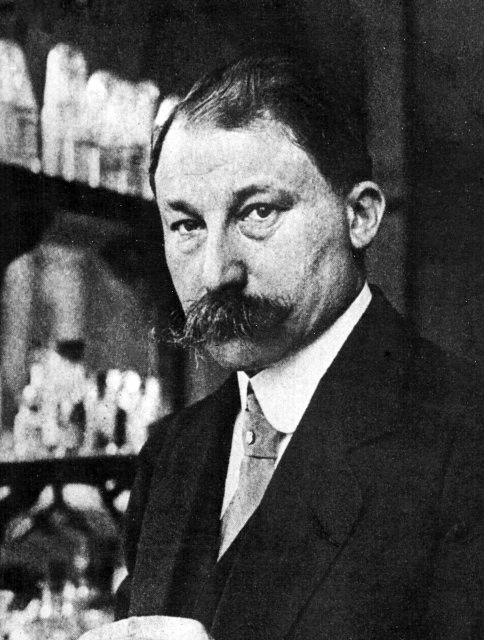
\includegraphics[width=\linewidth]{images/book2/grignard.jpg}
\end{minipage}\hfill
\begin{minipage}[t]{0.76\linewidth}\vspace{0pt}
O reagente leva o nome de Victor Grignard, que, como doutorando na
virada do século vinte, descobriu que o magnésio se dissolve em uma
solução de um haloalcano em éter e que essa solução se adiciona aos
compostos carbonílicos. Sua simplicidade --- um metal, um solvente, um
balão --- fez dela a reação de formação de ligações carbono--carbono
mais usada do século, e valeu a seu descobridor um Prêmio Nobel de
Química. (Fotografia, domínio público, Wikimedia Commons.)
\end{minipage}
\end{history}

\section{Exercícios}

\begin{exercise}[$\star$]\label{exo:b1:organomagnesium:1}
Escreva a preparação do brometo de etilmagnésio e do brometo de
fenilmagnésio. Dê a polarização da ligação C--Br e da ligação C--Mg, com
as \omterm{def:b1:periodicity:electronegativity}{eletronegatividades}.
\end{exercise}

\begin{exercise}[$\star$]\label{exo:b1:organomagnesium:2}
O que dá o iodeto de metilmagnésio com: água; etanol; ácido etanoico;
óxido de deutério \ce{D2O}? Escreva as equações.
\end{exercise}

\begin{exercise}[$\star$]\label{exo:b1:organomagnesium:3}
Dê o produto (após tratamento ácido) do brometo de etilmagnésio com
metanal, etanal, propanona, benzaldeído e dióxido de carbono. Dê a
classe de cada álcool.
\end{exercise}

\begin{exercise}[$\star$]\label{exo:b1:organomagnesium:4}
Por que o 4-bromobutan-1-ol não pode ser usado para preparar um \omterm{def:b1:organomagnesium:organometallic}{reagente
de Grignard}?
\end{exercise}

\begin{exercise}[$\star\star$]\label{exo:b1:organomagnesium:5}
Escreva o mecanismo da adição do brometo de metilmagnésio ao etanal e
do tratamento, com \omterm{def:b1:electronic-effects:curly-arrow}{setas curvas}. O produto é \omterm{def:b1:stereochemistry-in-depth:stereocentre}{quiral}? Ele é obtido como
um único \omterm{def:b1:stereochemistry-in-depth:enantiomers}{enantiômero}? Por quê?
\end{exercise}

\begin{exercise}[$\star\star$]\label{exo:b1:organomagnesium:6}
Proponha duas maneiras de preparar o 3-metilpentan-3-ol a partir de um
\omterm{def:b1:organomagnesium:organometallic}{reagente de Grignard} e de uma cetona.
\end{exercise}

\begin{exercise}[$\star\star$]\label{exo:b1:organomagnesium:7}
Como você prepararia o ácido 2-metilpropanoico a partir do
2-bromopropano? Calcule a massa de ácido obtida a partir de
\qty{12.3}{g} de brometo com \omterm{def:b1:extent-q-and-k:fractional-extent}{rendimento} de \qty{70}{\percent} ($M$:
\ce{C3H7Br} \qty{123.0}{g/mol}, \ce{C4H8O2} \qty{88.0}{g/mol}).
\end{exercise}

\begin{exercise}[$\star\star$]\label{exo:b1:organomagnesium:8}
Um estudante descuidado prepara brometo de fenilmagnésio a partir de
\qty{0.0500}{mol} de bromobenzeno em um éter que contém \qty{0.18}{g} de
água. Que fração do reagente é destruída? Que produto se forma?
\end{exercise}

\begin{exercise}[$\star\star$]\label{exo:b1:organomagnesium:9}
A bifenila, \ce{C6H5-C6H5}, é um subproduto da preparação do brometo de
fenilmagnésio. Proponha como ela se forma, e por que a adição lenta do
bromobenzeno a um excesso de magnésio a limita.
\end{exercise}

\begin{exercise}[$\star\star\star$]\label{exo:b1:organomagnesium:10}
Planeje duas sínteses do 1-feniletan-1-ol a partir de um \omterm{def:b1:organomagnesium:organometallic}{reagente de
Grignard}, e uma síntese do 2-fenilpropan-2-ol. Para cada uma, dê o nome
do haleto que fornece o reagente.
\end{exercise}

\begin{exercise}[$\star\star\star$]\label{exo:b1:organomagnesium:11}
Explique por que o \omterm{def:b1:organomagnesium:organometallic}{reagente de Grignard} e o composto carbonílico devem
ser misturados na ordem escolhida no problema abaixo, e por que o
tratamento é feito com ácido diluído frio, e não só com água.
\end{exercise}

\begin{exercise}[$\star\star\star$]\label{exo:b1:organomagnesium:12}
Um \omterm{def:b1:organomagnesium:organometallic}{reagente de Grignard} preparado a partir de \qty{0.100}{mol} de um
brometo é titulado: uma alíquota é derramada em excesso de água, e o sal
básico de magnésio formado é titulado por ácido clorídrico: referidos à
solução inteira, são necessários \qty{0.088}{mol} de ácido. Explique o
princípio e dê o \omterm{def:b1:extent-q-and-k:fractional-extent}{rendimento} da preparação.
\end{exercise}

\section{Problema: O trifenilmetanol}

\begin{problem}[{Problema de fim de semana --- a preparação do brometo de
fenilmagnésio, sua adição à benzofenona, o tratamento e o rendimento em
trifenilmetanol}]
\label{pb:b1:organomagnesium:1}
Em um balão de três bocas seco, \qty{0.535}{g} de magnésio e
\qty{3.14}{g} de bromobenzeno em etoxietano anidro dão brometo de
fenilmagnésio. Uma solução de \qty{3.28}{g} de benzofenona,
\ce{(C6H5)2CO}, no mesmo éter é então adicionada gota a gota. Após
tratamento com ácido sulfúrico diluído frio, extração e
recristalização, obtêm-se \qty{3.75}{g} de trifenilmetanol puro,
\ce{(C6H5)3COH}, e separam-se \qty{0.15}{g} de bifenila. Massas molares
(\unit{g/mol}):
Mg 24.3, \ce{C6H5Br} 156.9, \ce{C13H10O} 182.0, \ce{C19H16O} 260.0,
\ce{C12H10} 154.0, \ce{C7H6O2} 122.0.

\medskip
\noindent\textbf{Parte I --- O brometo de fenilmagnésio.}
\begin{enumerate}
  \item Escreva a equação da preparação.
  \item Calcule as quantidades de magnésio e de bromobenzeno. Qual está
        em excesso?
  \item Por que a aparelhagem precisa estar seca? Escreva a reação com a
        água.
  \item Qual é o papel do tubo secante?
  \item Por que o éter é essencial, além de dissolver os reagentes?
  \item A bifenila vem da reação do reagente com o bromobenzeno.
        Escreva-a e calcule a quantidade de bromobenzeno perdida com ela.
\end{enumerate}

\medskip
\noindent\textbf{Parte II --- A adição.}
\begin{enumerate}[resume]
  \item Calcule a quantidade de benzofenona.
  \item Escreva o mecanismo da adição com \omterm{def:b1:electronic-effects:curly-arrow}{setas curvas}.
  \item Que reagente limita a formação do trifenilmetanol? Leve em conta
        a Parte I.
  \item O trifenilmetanol é \omterm{def:b1:stereochemistry-in-depth:stereocentre}{quiral}? Justifique.
  \item Por que a benzofenona é adicionada ao reagente, e não o inverso?
  \item O que faria um traço de água na solução de benzofenona?
\end{enumerate}

\medskip
\noindent\textbf{Parte III --- O tratamento.}
\begin{enumerate}[resume]
  \item Escreva a protonação do alcóxido.
  \item Por que usar ácido diluído frio, e não só água?
  \item Onde ficam o trifenilmetanol e os sais de magnésio após a
        extração com éter?
  \item Como a bifenila é separada do trifenilmetanol? (A bifenila é muito
        mais solúvel em éter de petróleo frio.)
  \item Que teste confirma a pureza dos \omterm{def:b1:crystals-metals:crystal}{cristais}?
  \item O trifenilmetanol resiste ao ácido diluído frio, mas se dissolve
        no ácido sulfúrico concentrado dando um \omterm{def:b1:electronic-effects:intermediates}{carbocátion} amarelo
        intenso. Escreva sua formação e explique sua estabilidade
        (compare com o
        \cref{ch:b1:electronic-effects}).
\end{enumerate}

\medskip
\noindent\textbf{Parte IV --- \omterm{def:b1:extent-q-and-k:fractional-extent}{Rendimento} e outro produto.}
\begin{enumerate}[resume]
  \item Calcule a quantidade de trifenilmetanol obtida.
  \item Calcule o \omterm{def:b1:extent-q-and-k:fractional-extent}{rendimento} em relação ao \omterm{def:b1:extent-q-and-k:max-extent}{reagente limitante}.
  \item Sugira duas causas de perda.
  \item Se o reagente da Parte I (corrigido pela bifenila) tivesse sido
        derramado sobre dióxido de carbono sólido, que produto se
        formaria?
  \item Calcule a massa teórica desse produto.
  \item Escreva a equação dessa carboxilação.
  \item Indique o \omterm{def:b1:extent-q-and-k:fractional-extent}{rendimento} em trifenilmetanol, em porcentagem.
\end{enumerate}
\end{problem}
